%++++++++++++++++++++++++++++++++++++++++
\documentclass[letterpaper,11pt]{article}
\usepackage{natbib}
\usepackage[utf8]{inputenc}
\bibliographystyle{unsrtnat}
\usepackage{tabularx}
\usepackage{amsmath}
\usepackage{graphicx}
\usepackage[margin=1in,letterpaper]{geometry}
\usepackage[spanish]{babel}
\usepackage[final]{hyperref}
\hypersetup{
	colorlinks=true,      
	linkcolor=blue,        
	citecolor=blue,    
	filecolor=magenta,
	urlcolor=blue         
}
\renewcommand{\labelenumi}{[\arabic{enumi}]}
%+++++++++++++++++++++++++++++++++++++++
\begin{document}

% PORTADA
\thispagestyle{empty}
	
	\begin{figure}[ht]
	   \minipage{0.76\textwidth}
			
\includegraphics[width=4cm]{./img/LogoUGRLargo.png}
	   \endminipage
	   \minipage{0.32\textwidth}
			
\includegraphics[width=4cm]{./img/LogoFacultadCiencias.jpeg}
		\endminipage
	\end{figure}
	
	\begin{center}
	\vspace{0.8cm}
	\LARGE
	Universidad de Granada
	
	\vspace{0.8cm}
	\LARGE
	Facultad de Ciencias
	
	\vspace{1.7cm}	
	\Large
	\textbf{Práctica Evaluable: Aprendiendo de los datos}

	\vspace{1.3cm}
	\normalsize	
	PRESENTA \\
	\vspace{.3cm}
	\large
	\textbf{Juan Antonio Villegas Recio \\ i62virej@correo.ugr.es}
	
	\vspace{1.3cm}
	\normalsize	
	PROFESOR \\
	\vspace{.3cm}
	\large
	\textbf{José Luis Romero Béjar}
	
	\vspace{1.3cm}
	\normalsize	
	ASIGNATURA \\
	\vspace{.3cm}
	\large
	\textbf{Estadística Multivariante}
	
	\vspace{1.3cm}
	\normalsize	
	CURSO ACADÉMICO \\
	\vspace{.3cm}
	\large
	\textbf{2021/2022}
	
	\vspace{1.3cm}
	\today
	\end{center}
	
	\newpage
	

% DOCUMENTO

\title{Estadística Multivariante \\\textbf{Práctica Evaluable: Aprendiendo de los datos}}
\author{Juan Antonio Villegas Recio}
\date{\today}
\maketitle

\begin{abstract}

A partir de una base de datos con información variada de una serie de países, se pretende realizar un análisis exploratorio de los datos y descubrir posibles relaciones entre las variables y los países. Contamos con información como la densidad de población, el porcentaje de población activa, población urbana o libros publicados en cada país. Las variables con las que contamos de hecho son muy diversas en cuanto a contexto, por ello interesa buscar posibles relaciones entre variables. 

Para ello se han preprocesado los datos mediante la corrección de valores perdidos y valores extremos y utilizado técnicas de análisis univariante como tests de normalidad, gráficos \textit{boxplot} o \textit{qqplot}; multivariantes como análisis de componentes principales o análisis factorial junto con herramientas de aprendizaje automático como análisis de clusters. En conjunto, se busca con todas estas técnicas extraer la información de interés humano subyacente a este conjunto de datos, buscando con qué variables obtener la mayor cantidad de información, cuáles son más importantes, y posibles variables latentes subyacentes.
 
\end{abstract}

\section{Introducción}

Partimos de una base de datos con información sobre países de la cual se pretende extraer información relevante. Sin embargo, el conjunto de datos en crudo no está `limpio', en el sentido de que contiene algunos datos perdidos (`\textit{missing values}') y también datos anómalos, extremos o `\textit{outliers}'. Por lo que lo primero a lo que se procede es a limpiar el conjunto de datos los valores perdidos, para posteriormente realizar un profundo análisis descriptivo de cada variable. Tras este paso se eliminarán los \textit{outliers} y se procederá al análisis multivariante.

Como hemos dicho anteriormente, hay variables muy distintas pertenecientes a varios contextos diferentes: medicina, esperanza de vida, población urbana, población activa, consumo, etc. Esta diversidad nos sugiere estudiar posibles agrupaciones de variables inesperadas. Para ello se ha hecho uso de técnicas como el análisis factorial. También podemos buscar reducir la dimensión conservando la mayor parte de la información, y para ello aplicamos análisis de componentes principales, en ambos casos cerciorandonos previamente de los requisitos que las técnicas requieren. Por último, se ha aplicado una conocida técnica de aprendizaje automático no supervisado: el \textit{clustering}, buscando agrupaciones entre países que puedan ser significativas.

Por tanto, buscamos estudiar a fondo los datos que se nos dan, apreciando la distribución de cada variable por separado, para posteriormente estudiar la distribución multivariante. Se pretende buscar además agrupaciones de variables relacionadas junto con agrupaciones de instancias con características similares, haciendo así por tanto un estudio de variables relacionadas y de instancias con rasgos comunes en lo que a las variables con las que contamos respecta.

\section{Materiales y Métodos}

\subsection{Materiales}

Nuestro conjunto de datos cuenta con un total de 34 instancias, las cuales representan cada una un país del mundo. Hay representación de países de cada continente, con la variedad que eso implica a todos los niveles. El conjunto de datos cuenta además con 12 variables de las cuales 11 son numéricas y la restante es categórica: el nombre del país, por lo que claramente hay tantos valores como instancias y esta variable será excluida de los cálculos por tratarse principalmente de un identificador. Las variables numéricas están ya normalizadas con media 0 y varianza 1, teniendo así de antemano solucionados posibles problemas relacionados con las distintas escalas. Estas variables son:

\begin{itemize}
    \item \textbf{ZTLIBROP}: Número de libros publicados.
    \item \textbf{ZTEJERCI}: Cociente entre el número de individuos en ejército de tierra y población total del estado.
    \item \textbf{ZTPOBACT}: Cociente entre población activa y total.
    \item \textbf{ZTENERGI}: Tasa de consumo energético.
    \item \textbf{ZPSERVI}: Población del sector servicios.
    \item \textbf{ZPAGRICU}: Población del sector agrícola.
    \item \textbf{ZTMEDICO}: Tasa de médicos por habitante.
    \item \textbf{ZESPVIDA}: Esperanza de vida.
    \item \textbf{ZTMINFAN}: Tasa de mortalidad infantil.
    \item \textbf{ZPOBDENS}: Densidad de población.
    \item \textbf{ZPOBURB}: Porcentaje de población urbana.
\end{itemize}

En la tabla \ref{summary} podemos ver algunos estadísticos descriptivos de estas variables. Nótese que la media y la desviación típica de todas ellas son $0$ y $1$, respectivamente. Esto se debe y de hecho confirma que las variables están normalizadas. Para aportar algo de información relevante y descriptiva, podemos observar la mediana, el mínimo valor y el máximo.

\begin{table}[]
\centering
\renewcommand{\tablename}{Tabla}
\begin{tabular}{ccclll}
\hline
                  & \textbf{Media} & \textbf{Desviación típica} & \textbf{Mediana} & \textbf{Mínimo} & \textbf{Máximo} \\ \hline
\textbf{ZPOBDENS} & 0              & 1                          & -0.1616          & -1.0778         & 2.8616          \\ 
\textbf{ZTMINFAN} & 0              & 1                          & -0.3931          & -1.1026         & 1.9048          \\ 
\textbf{ZESPVIDA} & 0              & 1                          & 0.2781           & -2.1453         & 1.2486          \\ 
\textbf{ZPOBURB}  & 0              & 1                          & 0.1268           & -1.7697         & 1.5096          \\ 
\textbf{ZTMEDICO} & 0              & 1                          & -0.2916          & -1.1473         & 2.3717          \\ 
\textbf{ZPAGRICU} & 0              & 1                          & -0.2134          & -1.2342         & 1.9052          \\ 
\textbf{ZPSERVI}  & 0              & 1                          & 0.03541          & -1.88521        & 1.62885         \\ 
\textbf{ZTLIBROP} & 0              & 1                          & -0.2442          & -0.9696         & 2.4024          \\ 
\textbf{ZTEJERCI} & 0              & 1                          & -0.20626         & -0.86586        & 4.42620         \\ 
\textbf{ZTPOBACT} & 0              & 1                          & -0.1067          & -2.1341         & 1.7045          \\ 
\textbf{ZTENERGI} & 0              & 1                          & -0.39            & -0.9507         & 2.7498     		\\ \hline    
\end{tabular}
\caption{Estadísticos descriptivos de las variables}
\label{summary}
\end{table}

\subsection{Métodos estadísticos}

Sobre este conjunto de datos se han aplicado varias técnicas de análisis exploratorio de datos. Antes de utilizar técnicas más sofisticadas de análisis multivariante debemos imputar los \textbf{datos perdidos}. Una vez se tiene un conjunto de datos de calidad sin datos perdidos, es necesario hacer un estudio de cada variable para entender bien el contexto univariante en el que estamos trabajando.

Para ello, para cada variable se han calculado distintos coeficientes más extendidos que los ya comentados en el apartado anterior. Por ejemplo, medidas de centralidad resistente como la trimedia, de dispersión clásica como el rango, dispersión resistente como el rango intercuartílico, y de forma como los coeficientes de simetría. Únicamente con esta información podríamos hacernos una idea de la distribución que sigue cada variable. Sin embargo se ha graficado también un histograma tipo gráfico de barras agrupando los valores que toman las variables en intervalos de longitud 0.5 (véase figura \ref{histograma}). Este gráfico nos permite comprobar de forma visual los coeficientes numéricos calculados. 

\begin{figure}
\begin{center}
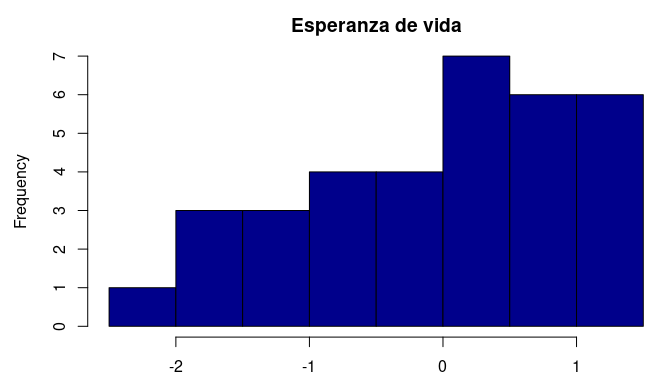
\includegraphics[scale=0.4]{./img/histograma.png}
\end{center}
\caption{Ejemplo de los histogramas utilizados}
\label{histograma}
\end{figure}

Una vez estudiadas las variables, en ciertos casos puede observarse la presencia de \textbf{valores anómalos}, por lo que también se modificaron los valores extremos de cada variable, importándolos por la media.

Seguidamente, con ayuda de gráficos \textit{qqplot} contrastamos visualmente la posible \textbf{normalidad de las variables}, para posteriormente estudiar la \textbf{homocedasticidad} entre ellas. Para estudiar la homocedasticidad entre posibles grupos introdujimos una nueva variable categórica: el continente. De esta forma, estudiamos la homocedasticidad entre los paises de Europa, Asia y África. En este punto del estudio, tenemos datos limpios y normalizados, listos para el análisis multivariante. 

Previo a la aplicación de técnicas multivariantes, contrastamos mediante la matriz de correlación que los datos están correlados, requisito en la aplicación de las técnicas que aplicamos posteriormente: el análisis de componentes y el análisis factorial. Aplicamos el \textbf{análisis de componentes principales} para poder extraer a partir de él las combinaciones lineales de variables que aportan mayor varianza explicada, pudiendo reducir la dimensión sin perder gran cantidad de información. Sobre el \textbf{análisis factorial}, buscamos explicar posibles variables latentes en base a distintos factores subyacentes al conjunto de datos.

Por último, y dado que el conjunto de datos no posee variable categórica susceptible de aplicar ninguna técnica de aprendizaje supervisado, le aplicamos una técnica conocida de aprendizaje no supervisado: el \textbf{clustering}, agrupando así las distintas instancias de nuestro conjunto de datos en distintos grupos con características similares.

\section{Resultados}

Antes de exponer los resultados, debe comentarse que se debe tener en cuenta que el conjunto de datos es muy pequeño, sólo contiene 34 instancias, lo cual hace que algunos métodos no funcionen del todo bien y no se extraigan conclusiones realmente esperadas.

Dicho esto, tras un análisis univariante en el que conocimos la distribución y las características más relevantes de una variable, presentamos a continuación en la figura \ref{boxplot} una comparativa de boxplot de las distintas variables antes y después de eliminar datos perdidos y \textit{outliers}. Como podemos observar se eliminaron los \textit{outliers} existentes en todas las variables. Además, a partir de los gráficos podemos hacernos a una idea de la distribución de los distintos atributos numéricos.

\begin{figure}[h]
\begin{tabular}{cc}
  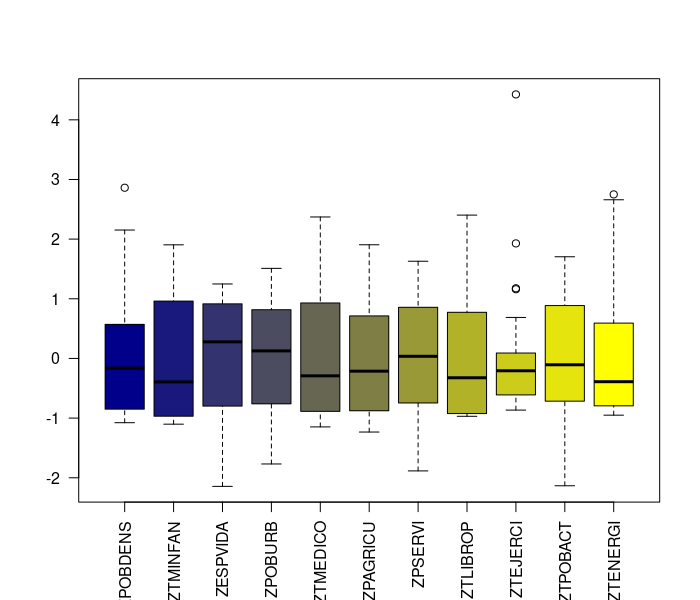
\includegraphics[scale=0.4]{./img/boxplot_enteros.png} &   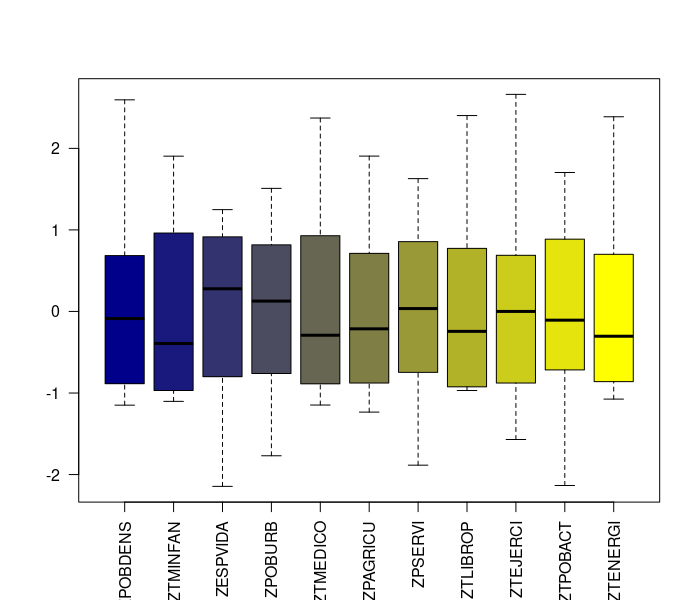
\includegraphics[scale=0.4]{./img/boxplot_procesados.png} \\
(a) Datos en crudo & (b) Datos procesados \\[6pt]
\end{tabular}
\caption{Boxplot de las variables previo y posterior al preprocesado}
\label{boxplot}
\end{figure}

Con ayuda de los gráficos \textit{qqplot} de la figura \ref{qqplot} pudimos hacernos una primera idea de qué variables se aproximan realmente a una normal.

\newpage

\begin{figure}[h]
\begin{center}
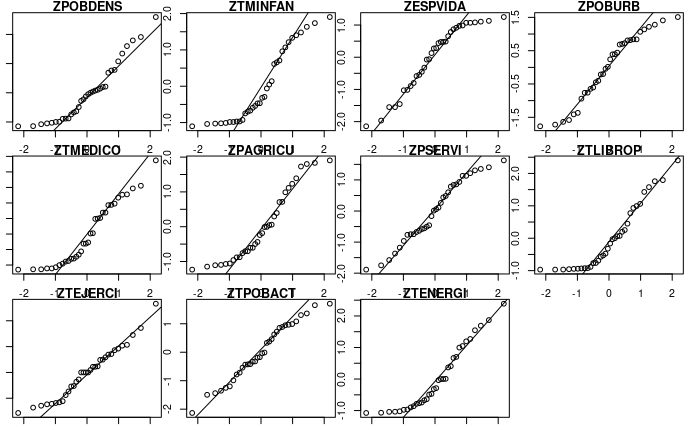
\includegraphics[scale=0.5]{./img/qq.png}
\end{center}
\caption{Ejemplo de los qqplot utilizados}
\label{qqplot}
\end{figure}

Observamos que la mayoría de las variables tienden a acercarse a la diagonal, por ejemplo, \textbf{ZPOBURB} (fila 1, columna 4) y \textbf{ZTPOBACT} (fila 3, columna 2) se aproximan mucho a la diagonal. Sin embargo, \textbf{ZPOBDENS} (fila 1, columna 1) y \textbf{ZTMINFAN} (fila 1, columna 2) se alejan más de la diagonal, y por tanto de la distribución normal.

Por otra parte, al comprobar la homocedasticidad con respecto al continente, se obtuvo que \textbf{para todas las variables salvo para ZPOBURB y ZESPVIDA había homocedasticidad} entre los países de Europa, de Asia y de África.

Seguidamente, se estudió la posible correlación entre las variables, contrastando mediante el `test de Bartlett' si la matriz de correlaciones era la identidad o no. En la imagen \ref{correlaciones} podemos observar un heatmap representativo de la matriz de correlaciones, en el que comprobamos visualmente que la matriz no se parece en nada a una matriz identidad. De todas formas, el propio test de Barlett nos devolvió un p-valor de $1.14\times 10^{-232}$, prácticamente nulo, por lo que \textbf{podemos asumir que en efecto las variables están correladas}.

\begin{figure}
\begin{center}
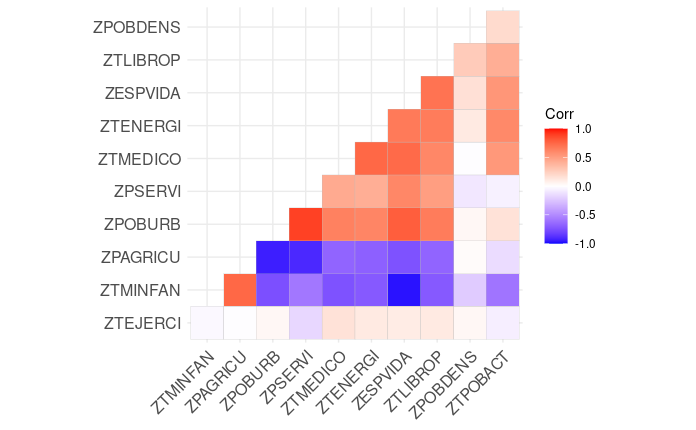
\includegraphics[scale=0.6]{./img/correlaciones.png}
\end{center}
\caption{Heatmap de la matriz de correlaciones}
\label{correlaciones}
\end{figure}

Una vez tenemos datos correlados, completos y sin outliers, procedemos a aplicar las técnicas multivariantes de reducción de la dimensión. Comenzamos por el \textbf{Análisis de componentes principales}. Mostramos una tabla con un resumen de las varianzas y las varianzas explicadas de las distintas componentes principales (tabla \ref{ACP_tabla}). Sin embargo, el resumen más visual son gráficos de la figura \ref{ACP_grafico}, en los que se puede observar el porcentaje de varianza explicada (a) por cada componente principal junto con el porcentaje de varianza acumulada (b).

\begin{table}[]
\centering
\renewcommand{\tablename}{Tabla}
\begin{tabular}{lllll}
\hline
     & Desviación típica & Varianza   & Varianza explicada & Varianza acumulada \\ \hline
PC1  & 2.4818            & 6.15934602 & 0.5599             & 0.5599             \\
PC2  & 1.2806            & 1.63988972 & 0.1491             & 0.7090             \\
PC3  & 1.03112           & 1.06319852 & 0.09665            & 0.80568            \\
PC4  & 0.95154           & 0.90543213 & 0.08231            & 0.88799            \\
PC5  & 0.6448           & 0.41577420 & 0.0378            & 0.9258            \\
PC6  & 0.60272           & 0.36326910 & 0.03302            & 0.95881            \\
PC7  & 0.48187            & 0.23219856 & 0.02111             & 0.97992             \\
PC8  & 0.33542           & 0.11250601  & 0.01023            & 0.99015            \\
PC9  & 0.24916           & 0.06208202 & 0.00564            & 0.99579            \\
PC10 & 0.16420           & 0.02696079 & 0.00245            & 0.99824            \\
PC11 & 0.13908           & 0.01934294 & 0.00176            & 1                  \\ \hline
\end{tabular}
\caption{Estadísticos de las componentes principales}
\label{ACP_tabla}
\end{table}

\begin{figure}
\begin{tabular}{cc}
  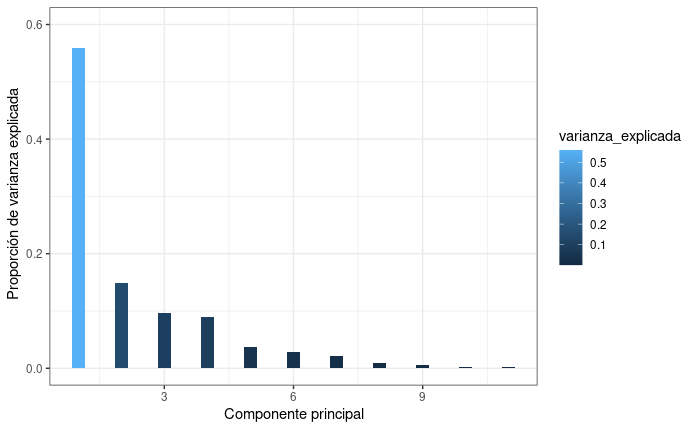
\includegraphics[scale=0.4]{./img/ACP_explicada.png} &   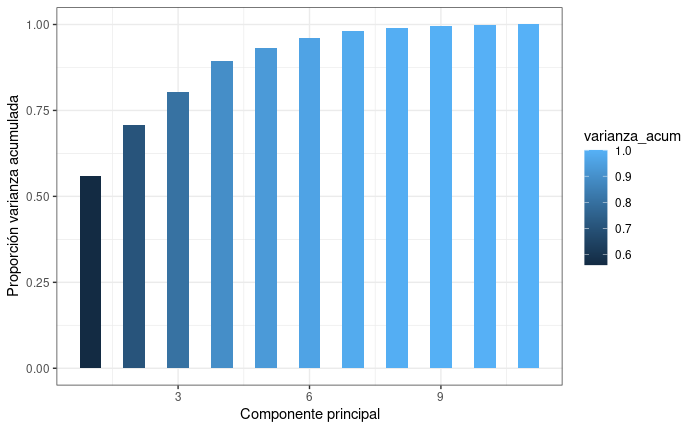
\includegraphics[scale=0.4]{./img/ACP_acumulada.png} \\
(a) Varianza explicada & (b) Varianza acumulada \\[6pt]
\end{tabular}
\caption{Gráficos de la varianza explicada y acumulada por cada CP}
\label{ACP_grafico}
\end{figure}

Seguidamente debíamos especificar el número óptimo de componentes principales, para ello utilizamos el la regla de Abdi et al. (2010): se promedia las varianzas explicadas por la componentes principales y se seleccionan aquellas cuya proporción de varianza explicada supera la media. La media de las varianzas de las componentes principales es 1, por lo que se seleccionaron las \textbf{3 primeras componentes principales}. Por último, en la figura \ref{ACP_variables} vemos unos gráficos que nos mostrarán la influencia de cada variable en cada componente principal de manera visualmente interpretable.

\begin{figure}[]
\begin{tabular}{cc}
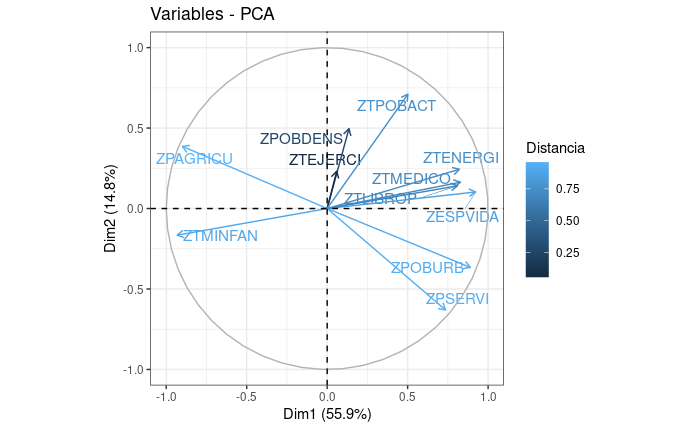
\includegraphics[scale=0.4]{./img/ACP_PC12.png} & 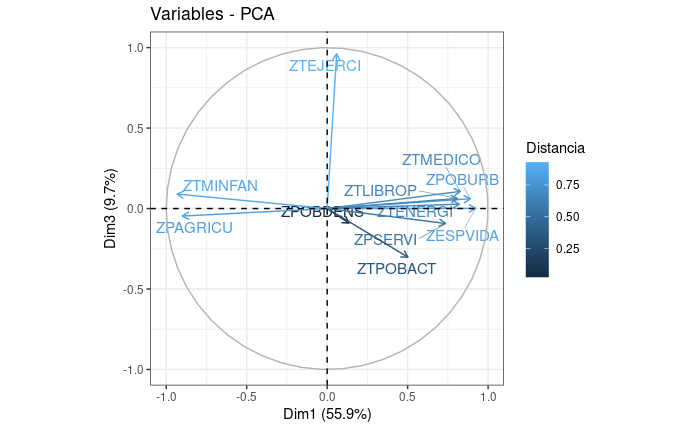
\includegraphics[scale=0.4]{./img/ACP_PC13.png} \\
(a) Componentes 1 y 2 & (b) Componentes 1 y 3 \\[6pt]
\multicolumn{2}{c}{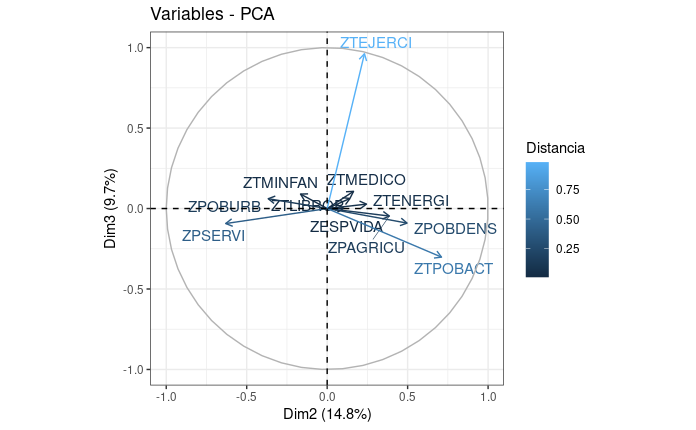
\includegraphics[scale=0.4]{./img/ACP_PC23.png}} \\
\multicolumn{2}{c}{(c) Componentes 2 y 3 }

\end{tabular}
\caption{Influencia de las variables en las tres primeras componentes}
\label{ACP_variables}
\end{figure}

Una vez expuestos los resultados correspondientes al análisis de componentes principales, expondremos los resultados que nos ofreció la técnica del análisis factorial. Primero de todo es necesario fijar el número óptimo de factores a fijar en el análisis, y para ello nos ayudamos del gráfico conocido en la literatura como `\textit{scree plot}' (figura \ref{AF} (a)), donde el número de puntos antes de un cambio en la tendencia comúnmente llamado `codo' nos dice el número óptimo de factores. Sin embargo, en este caso se intuye que el número óptimo debe estar entre 2 y 3 factores, pero no se puede concluir a partir del gráfico, aunque a partir de un test chi cuadrado se pudo concluir que \textbf{el número óptimo de factores es 3}.

\begin{figure}
\begin{tabular}{cc}
  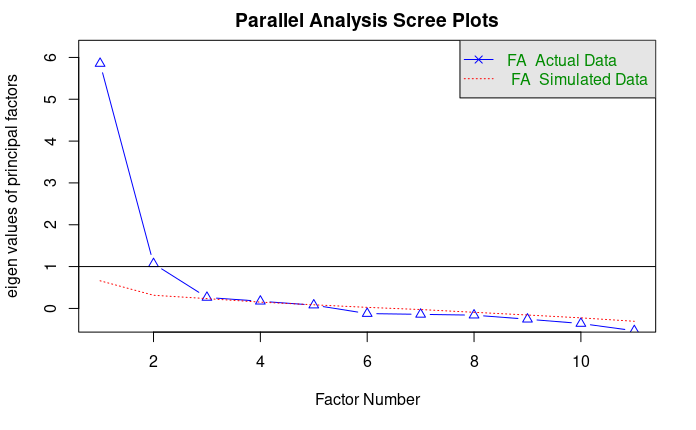
\includegraphics[scale=0.4]{./img/codo.png} &   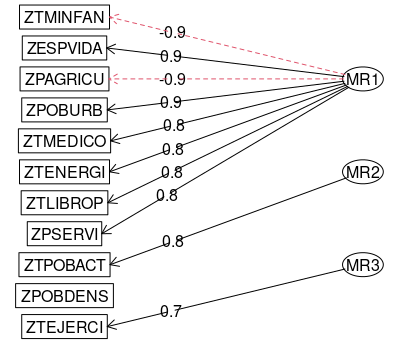
\includegraphics[scale=0.5]{./img/AF.png} \\
(a) \textit{Scree plot} & (b) Agrupación de variables tras el AF \\[6pt]
\end{tabular}
\caption{Scree plot y agrupación de variables en el análisis factorial}
\label{AF}
\end{figure}

Por tanto, podemos calcular un modelo al cual no le hemos aplicado ninguna rotación. La agrupación de las variables resultante se puede ver en el gráfico \ref{AF} (b).

La última técnica de análisis exploratorio que aplicamos fue el análisis de clusters, conocido en minería de datos simplemente como clustering. Decidimos aplicar el algoritmo `\textit{K-Medias}', aunque dicho algoritmo tiene el defecto de que necesita prefijar un número de clusters a crear, desconociendo a priori cual es el óptimo. La elección se hizo en base al método de la silueta, en el cual aplicamos varios valores distintos y nos quedamos con el que ofrezca mejor coeficiente \textit{silhouette}. En otras palabras, el número que nos ofrezca una agrupación de mayor calidad. Si nos fijamos entonces en el gráfico \ref{silhouette}, podemos concluir que \textbf{el número óptimo de clusters es 2}.

\begin{figure}
\begin{center}
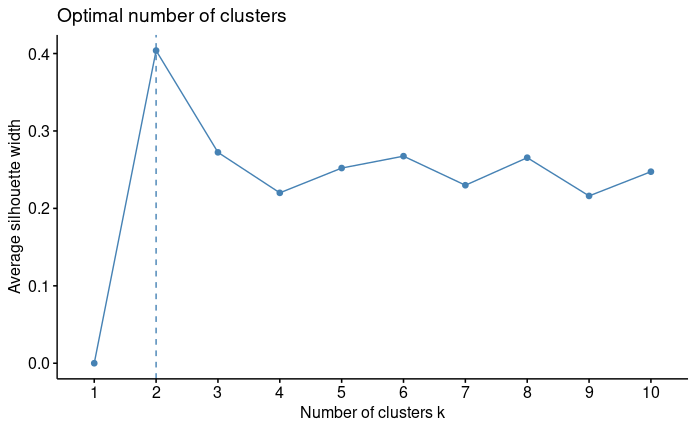
\includegraphics[scale=0.4]{./img/silhouette.png}
\end{center}
\caption{Gráfico de los coeficientes \textit{silhouette} según parámetro $k$}
\label{silhouette}
\end{figure}

\newpage

Por tanto, aplicamos \textit{K-Medias} con el parámetro $k=2$, obteniendo la agrupación que podemos ver en la figura \ref{clustering}.

\begin{figure}[h]
\begin{center}
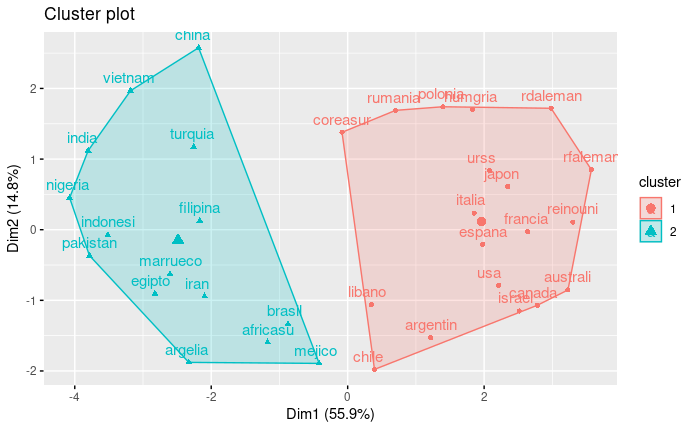
\includegraphics[scale=0.7]{./img/clustering.png}
\end{center}
\caption{Clustering calculado por \textit{K-Medias}}
\label{clustering}
\end{figure}

\section{Discusión}

Para el análisis de los resultados obtenidos, recordamos que el conjunto de datos no está realmente preparado para todas las técnicas empleadas, por lo que unas pueden darnos alguna conclusión de interés y otras pueden no aportar gran cosa.

Comenzamos examinando los resultados del análisis de componentes principales. En los gráficos de la figura \ref{ACP_grafico} podemos observar que ya con la primera componente principal se obtiene un alto porcentaje de la varianza explicada, por lo que combiene fijarse en las variables que mayor influencia tienen en esta primera componente principal. Estas son las que consiguen que se explique un alto porcentaje de varianza total, concretamente, un 55.9\%. Aunque la primera componente principal tiene un alto porcentaje, la conclusión fue que debemos observar un total de 3 componentes principales, y estas tres primeras componentes explican en conjunto un 80.5\% de la varianza total. Veamos qué variables tienen mayor influencia en estas tres primeras componentes principales.

Para ver de qué variables hablamos, recurrimos a los gráficos de la figura \ref{ACP_variables}. Como vemos, en la primera componente principal (gráficos (a) y (b)) la mayoría de las variables tienen peso (flechas horizontales), aunque destacamos a \textbf{ZPOBDENS} y a \textbf{ZTEJERCI} que no parecen tener tanto peso, las flechas son más verticales. Mientras que si observamos la tercera componente principal (gráficos (b) y (c)), vemos que \textbf{ZTEJERCI} tiene más peso en la tercera componente principal, mientras que \textbf{ZPOBDENS} tiende a repartirlo entre las tres componentes principales, sin llegar a tener demasiado en ninguna de las 3, pues su mayor peso se encontraba en la cuarta componente principal.

Discutido el análisis de componentes principales, veamos qué nos ofrece el análisis factorial. De un primer vistazo, utilizando el mapa de calor de la matriz de correlaciones ordenando correctamente las variables, tal y como podemos observar en el gráfico de la figura \ref{correlaciones_AF}, podemos ver una agrupación de círculos grandes e intensos entre las variables que finalmente formaron el primer factor: \textbf{ZPAGRICU}, \textbf{ZPOBURB}, \textbf{ZPSERVI}, \textbf{ZESPVIDA}, \textbf{ZTMINFAN}, \textbf{ZTLIBROP}, \textbf{ZTMEDICO} y \textbf{ZTENERGI}. Por su parte, \textbf{ZPOBACT}, \textbf{ZTEJERCI} y \textbf{ZTEJERCI} no parecen tener correlaciones fuertes. Si volvemos a fijarnos en la figura \ref{AF} (b), vemos que \textbf{ZTPOBACT} y \textbf{ZTEJERCI} formaban un factor por sí solas mientras que \textbf{ZPOBDENS} no entraba en ningún factor. Esto nos dice que estas tres variables tienen muy poca relación con las demás, son poco relevantes. Comentamos además que precisamente \textbf{ZPOBDENS} tenía mayor peso en la cuarta componente principal mientras que \textbf{ZTEJERCI} lo tenía en la segunda.

\begin{figure}[h]
\begin{center}
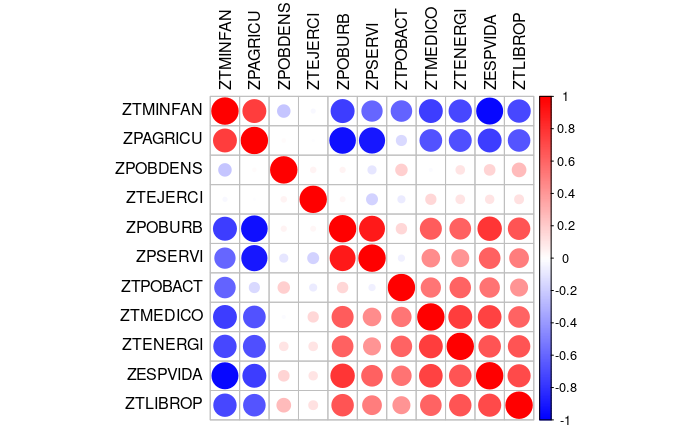
\includegraphics[scale=0.6]{./img/correlaciones_AF.png}
\end{center}
\caption{\textit{Heatmap} de correlaciones}
\label{correlaciones_AF}
\end{figure}


\begin{table}[h]
\centering
\renewcommand{\tablename}{Tabla}
\begin{tabular}{ccc}
\hline
                  & \textbf{Cluster 1} & \textbf{Cluster 2} \\ \hline
\textbf{ZPOBDENS} & 0.204303116633573  & -0.229841006212769 \\
\textbf{ZTMINFAN} & -0.785394103948831 & 0.883568366942435  \\
\textbf{ZESPVIDA} & 0.776931624843956  & -0.87404807794945  \\
\textbf{ZPOBURB}  & 0.724059233362857  & -0.814566637533213 \\
\textbf{ZTMEDICO} & 0.767130858244767  & -0.863022215525363 \\
\textbf{ZPAGRICU} & -0.744880159181466 & 0.837990179079149  \\
\textbf{ZPSERVI}  & 0.595641464996393  & -0.670096648120943 \\
\textbf{ZTLIBROP} & 0.626969200299131  & -0.705340350336522 \\
\textbf{ZTEJERCI} & 0.149951897980828  & -0.168695885228432 \\
\textbf{ZTPOBACT} & 0.447433162619418  & -0.503362307946846 \\
\textbf{ZTENERGI} & 0.672556509553323  & -0.756626073247489 \\ \hline
\end{tabular}
\caption{Centroides de los clusters}
\label{AC_tabla}
\end{table}

Hasta el momento hemos hecho un análisis de las variables que parecen tener mayor relevancia en el conjunto de datos, evidenciando que las variables \textbf{ZPOBDENS}, \textbf{ZTEJERCI} y en menor medida \textbf{ZTPOBACT} son las menos relevantes dentro del conjunto de datos. Estudiadas las distintas características es momento de agrupar las instancias, y para ello utilizamos el análisis de clusters. Para ello utilizamos una tabla que reúne los centroides de los clusters, la tabla \ref{AC_tabla}. 

Llama la atención que en la mayoría de las variables un cluster tiene media positiva y el otro negativa, como si en un cluster se encontraran países con dicha medida alta y en el otro baja, y este patrón se repite en la mayoría de las variables. Si miramos de nuevo el gráfico \ref{clustering} podemos poner algún ejemplo: la población dedicada al sector agrícola es más alta en países como Nigeria o China que en USA o en Francia.

\section{Conclusión}

Tras los análisis y las discusiones, podemos concluir que del conjunto de datos que tenemos, las variables menos relevantes son \textbf{ZPOBDENS}, \textbf{ZTEJERCI} y \textbf{ZTPOBACT}, ya que son las que tienen no sólo menos relevancia en la primera y segunda componente principal, sino que han sido excluidas del primer factor en el análisis factorial. Por ello, las variables más relacionadas entre sí y más significativas son \textbf{ZPAGRICU}, \textbf{ZPOBURB},\textbf{ZPSERVI}, \textbf{ZESPVIDA}, \textbf{ZTMINFAN}, \textbf{ZTLIBROP}, \textbf{ZTMEDICO} y \textbf{ZTENERGI}, las variables del primer factor. Por otra parte, el análisis de clusters realmente no nos ha aportado mucho más allá de lo que ya sabíamos, aunque nos ayuda a realzar las grandes diferencias que hay entre países en los diversos aspectos que este conjunto de datos nos proporciona.

Sin embargo, el estudio está limitado por el tamaño reducido de la base de datos, que no es suficiente para concluir normalidad en las variables ni para sacar conclusiones demasiado fiables. Con un conjunto de datos mayor y gracias al teorema central del límite, podríamos tener una mayor certeza de que las variables se aproximan a una normal, pudiendo así además contar con todos los métodos que necesitan la asunción de normalidad.

Otra forma de abordar el estudio sería utilizando variables semánticamente más similares. Al pocas variables y muy distintas, el análisis factorial no ha conseguido sino únicamente excluir las menos relevantes, cuando su cometido real es agrupar variables observables en torno a factores latentes no observables.

\section{Bibliografía}
\begin{enumerate}

\item Béjar, JL. \textit{Diapositivas de Estadística Multivariante}.

\item Béjar, JL. \textit{Códigos de prácticas de Estadística Multivariante}.

\item colaboradores de Wikipedia. (2021, 23 abril). \textit{Prueba de Bartlett}. Wikipedia, la enciclopedia libre.

\item GeeksforGeeks. (2021, 30 abril). \textit{How to add a column based on other columns in R DataFrame ?} https://www.geeksforgeeks.org/how-to-add-a-column-based-on-other-columns-in-r-dataframe/

\item ggplot2 : \textit{Quick correlation matrix heatmap - R software and data visualization - Easy Guides - Wiki - STHDA}. (2021). STHDA. http://www.sthda.com/english/wiki/ggplot2-quick-correlation-matrix-heatmap-r-software-and-data-visualization

\item \textit{Glosarios especializados de Ciencias, Artes, Técnicas y Sociedad.} Glosarios especializados. https://glosarios.servidor-alicante.com/

\item Hoffman, K. (2021, 13 diciembre).\textit{ Customizable correlation heatmaps in R using purrr and ggplot2}. Medium. https://towardsdatascience.com/customizable-correlation-plots-in-r-b1d2856a4b05

\item \textit{How to change color scheme in corrplot}. Code Redirect. https://coderedirect.com/questions/404197/how-to-change-color-scheme-in-corrplot

\item Jaadi, Z. (2021, 1 diciembre). \textit{A Step-by-Step Explanation of Principal Component Analysis (PCA)}. Built In. https://builtin.com/data-science/step-step-explanation-principal-component-analysis

\item \textit{levene.test function} - RDocumentation. RDocumentation. https://www.rdocumentation.org/packages/lawstat/versions/3.4/topics/levene.test

\item Newest Questions. Stack Overflow. https://stackoverflow.com/questions/

\item \textit{PCA Job Description | Personal Care Aide}. (2017, 29 mayo). Community Home Health Care. https://commhealthcare.com/home-care-services/personal-care-aides-pca/pca-job-description/

\end{enumerate}



\end{document}
